\documentclass[a4paper, 12pt]{article}

\usepackage{arxiv}

\usepackage[T2A]{fontenc}
\usepackage[utf8]{inputenc}
\usepackage[english, russian]{babel}
% \usepackage{cmap}
\usepackage{url}
\usepackage{booktabs}
\usepackage{nicefrac}
\usepackage{microtype}
\usepackage{lipsum}
\usepackage{graphicx}
\usepackage{subfig}
\usepackage[square,sort,comma,numbers]{natbib}
\usepackage{doi}
\usepackage{multicol}
\usepackage{multirow}
\usepackage{tabularx}

\usepackage{tikz}
\usetikzlibrary{matrix}

% Algorithms
\usepackage{algpseudocode}
\usepackage{algorithm}

%% Шрифты
\usepackage{euscript} % Шрифт Евклид
\usepackage{mathrsfs} % Красивый матшрифт
\usepackage{extsizes} % Возможность сделать 14-й шрифт

\usepackage{makecell} % diaghead in a table
\usepackage{amsmath,amsfonts,amssymb,amsthm,mathtools,dsfont}
\usepackage{icomma}

\newcommand{\bz}{\mathbf{z}}
\newcommand{\bx}{\mathbf{x}}
\newcommand{\by}{\mathbf{y}}
\newcommand{\bv}{\mathbf{v}}
\newcommand{\bw}{\mathbf{w}}
\newcommand{\ba}{\mathbf{a}}
\newcommand{\bb}{\mathbf{b}}
\newcommand{\bp}{\mathbf{p}}
\newcommand{\bq}{\mathbf{q}}
\newcommand{\bt}{\mathbf{t}}
\newcommand{\bu}{\mathbf{u}}
\newcommand{\bs}{\mathbf{s}}
\newcommand{\bT}{\mathbf{T}}
\newcommand{\bX}{\mathbf{X}}
\newcommand{\bZ}{\mathbf{Z}}
\newcommand{\bS}{\mathbf{S}}
\newcommand{\bH}{\mathbf{H}}
\newcommand{\bW}{\mathbf{W}}
\newcommand{\bY}{\mathbf{Y}}
\newcommand{\bU}{\mathbf{U}}
\newcommand{\bQ}{\mathbf{Q}}
\newcommand{\bP}{\mathbf{P}}
\newcommand{\bA}{\mathbf{A}}
\newcommand{\bB}{\mathbf{B}}
\newcommand{\bC}{\mathbf{C}}
\newcommand{\bE}{\mathbf{E}}
\newcommand{\bF}{\mathbf{F}}
\newcommand{\bomega}{\boldsymbol{\omega}}
\newcommand{\btheta}{\boldsymbol{\theta}}
\newcommand{\bgamma}{\boldsymbol{\gamma}}
\newcommand{\bdelta}{\boldsymbol{\delta}}
\newcommand{\bPsi}{\boldsymbol{\Psi}}
\newcommand{\bpsi}{\boldsymbol{\psi}}
\newcommand{\bxi}{\boldsymbol{\xi}}
\newcommand{\bchi}{\boldsymbol{\chi}}
\newcommand{\bzeta}{\boldsymbol{\zeta}}
\newcommand{\blambda}{\boldsymbol{\lambda}}
\newcommand{\beps}{\boldsymbol{\varepsilon}}
\newcommand{\bZeta}{\boldsymbol{Z}}
% mathcal
\newcommand{\cX}{\mathcal{X}}
\newcommand{\cY}{\mathcal{Y}}
\newcommand{\cW}{\mathcal{W}}

\newcommand{\dH}{\mathds{H}}
\newcommand{\dR}{\mathds{R}}
% transpose
\newcommand{\T}{^{\mathsf{T}}}

% \renewcommand{\shorttitle}{\textit{arXiv} Шаблон}
\renewcommand{\epsilon}{\ensuremath{\varepsilon}}
\renewcommand{\phi}{\ensuremath{\varphi}}
\renewcommand{\kappa}{\ensuremath{\varkappa}}
\renewcommand{\le}{\ensuremath{\leqslant}}
\renewcommand{\leq}{\ensuremath{\leqslant}}
\renewcommand{\ge}{\ensuremath{\geqslant}}
\renewcommand{\geq}{\ensuremath{\geqslant}}
\renewcommand{\emptyset}{\varnothing}

\usepackage{hyperref}
% \usepackage[usenames,dvipsnames,svgnames,table,rgb]{xcolor}

\hypersetup{
	unicode=true,
	pdftitle={A template for the arxiv style},
	pdfsubject={q-bio.NC, q-bio.QM},
	pdfauthor={David S.~Hippocampus, Elias D.~Striatum},
	pdfkeywords={First keyword, Second keyword, More},
	colorlinks=true,
	linkcolor=black,        % внутренние ссылки
	citecolor=blue,         % на библиографию
	filecolor=magenta,      % на файлы
	urlcolor=blue           % на URL
}

\graphicspath{{../figures/}}

\usepackage{enumitem} % Для модификаций перечневых окружений

\theoremstyle{definition} % "Определение"
\newtheorem{definition}{Опр.}[section]

\usepackage{etoolbox}

\makeatletter
\expandafter\patchcmd\csname\string\algorithmic\endcsname{\itemsep\z@}{\itemsep=1.5mm}{}{}
\makeatother
\renewcommand{\abstractname}{Аннотация}

\title{Автоматическое выделение терминов для тематического моделирования}

\author{
	  Никитина Мария Александровна\\
	\texttt{nikitina.mariia@phystech.edu} \\
 \\
        \textbf{Консультант: Потапова Полина Сергеевна} \\
	\texttt{potapov.polina@gmail.com} \\
 \\
        \textbf{Эксперт: Доктор ф-м наук, Воронцов Константин Вячеславович} \\
}
\date{\today}

\begin{document}
\maketitle

\begin{abstract}
В данной статье рассматривается задача автоматического выделения терминов в коллекции документов. Новые научные термины появляются каждый день.
Ручное извлечение терминов с привлечением узукоспециализированных
специалистов является трудозатратным. Цель настоящей работы --- обнаружение таких терминов в коллекциях документов в автоматическом режиме. Для решения данной задачи используется метод выделения коллокаций (TopMine) в сочетании с модульной технологией тематического моделирования (с использованием библиотеки BigARTM) и современные методы, основанные на нейросетевых моделях языка. Производится сравнение рассматриваемых решений.
\end{abstract}

\keywords{тематическое моделирование \and TopMine \and BigARTM \and Automatic Term Extraction}

\section{Введение}

        Поиск научных терминов в коллекции документов вручную практически невозможен из-за слишком больших объёмов работы. Для экономии ресурсов и времени предлагается рассмотреть задачу автоматического выделения терминов. К её решению можно подойти с разных сторон. Например, использовать сочетание метода выделения коллокаций с технологией математического моделирования \citep{ElKishky2014}. \textit{Коллокация} -- слово или словосочетание, имеющее признаки синтаксически и семантически целостной единицы

        \textit{Тематическое моделирование} -- это технология обработки естественного языка, направленная на определение тем, к которым относится текстовый документ из коллекции, и какие слова каждую тему образуют. Иначе говоря, тематическая модель осуществляет \textit{мягкую кластеризацию}, выбирая для документа кластеры-темы.

        \textit{Вероятностная тематическая модель} определяет вероятности тем в каждом документе и вероятности слов в каждой теме. Большим отличием такой модели от глубоких нейронных сетей типа BERT \citep{bert} или GPT-3 \citep{Brown2020LanguageMA} является простота организации и свойство интерпретируемости в ущерб качеству предсказания вероятности появления слов в документе. Векторное представление тяжёлой нейросети всё ещё не удалось интерпретировать, в то время как тематический эмбединг -- это вектор вероятностей тем.

        Новизной данной статьи является сравнение этих двух подходов. Нейросеть использована готовая. 
        % Здесь нужно вставить, какую нейросеть используем.
        Для построения же тематической модели требуется подбор \textit{регуляризаторов} -- критериев, учитывающих специфические особенности данных или предметной области, от подбора которых значительно зависит качество определения основных тем документов. В данной работе используется модель \textit{аддитивной регуляризации тематической модели, ARTM} \citep{vorontsov2020}. Для построения тематической модели с аддитивной регуляризацией используется библиотека BigARTM \citep{Vorontsov2015} с открытым кодом.

        Перед выполнением кластеризации необходимо выделить из коллекции документов ключевые слова и словосочетания и отбросить те, что не несут основной смысловой нагрузки. Поиск составных терминов является нетривиальной и трудоёмкой задачей. Для её решения используется метод поиска коллокаций TopMine, использующий информацию о частоте и совстречаемости слов в коллекции \citep{shatalov2019}.

        % Ещё какая-то информация про датасеты

        С учётом интерпретируемости и простоты тематическая модель является хорошей заменой нейросети. Предшествующие исследования предлагаемого подхода показали хорошие результаты как по полноте, так и по вычислительной эффективности. В работе сравниваются тематическая модель и сложная нейросетевая модель, анализируется их качество для рассматриваемой задачи.

\section{Постановка задачи}

        Основная задача -- построение модели ATE (Automatic Term Extraction) для автоматического выделения словосочетаний, являющихся терминами предметной области, в текстах научных статей. Предлагается использовать эффективные методы выделения коллокаций и тематические модели для определения «тематичности» словосочетания. Модель должна обучаться без учителя.

        Для решения поставленной задачи применяются алгоритмы поиска коллокаций TopMine с последующей фильтрацией по критерию тематичности, подбор гиперпараметров тематической модели и критерия тематичности.

        Задача называется корректно поставленной по Адамару, если её решение существует, единственно и устойчиво. В общем случае построение тематической модели – некорректно поставленная задача по Адамару, поэтому её нужно дополнить регуляризаторами. В практических задачах автоматической обработки текстов существует очень много критериев и ограничений.

        Пусть $p_{\omega d}$ -- вероятность появления терма $\omega$ в документе $d$, $\phi_{\omega t}$ -- вероятность того, что терм $\omega$ относится к теме $t$, $\theta_{td}$ -- вероятность встречи темы $t$ в документе $d$. Тогда $P = (p_{\omega d})_{W \times D}$ -- матрица частот термов в документах, $\Phi = (\phi_{\omega t})_{W \times T}$ -- матрица термов тем, $\Theta = (\theta_{td})_{T \times D}$ -- матрица тем документов. $W$, $D$, $T$ -- множества всех термов, документов и тем соответственно.
       
        Аддитивная регуляризация тематических моделей основана на максимизации логарифма правдоподобия и регуляризаторов $R_i(\Phi, \Theta)$ с неотрицательными коэффициентами регуляризации $\tau_i$, $i = 1, ..., k$ \citep{vorontsov2020}:
        \begin{equation}
            \sum\limits_{d \in D}\sum\limits_{w \in d}\ln\sum\limits_{t \in T}\phi_{\omega t}\theta_{td} + R(\Phi, \Theta) \to \max\limits_{\Phi, \Theta}; ~~~~~ R(\Phi, \Theta) = \sum\limits_{i = 1}^k\tau_iR_i(\Phi, \Theta);
        \end{equation}
        при ограничениях неотрицательности и нормировки:
        \begin{equation}
            \sum\limits_{w \in W}\phi_{\omega t} = 1; ~~~ \phi_{\omega t} \geq 0; ~~~~~ \sum\limits_{t \in T}\theta_{td} = 1; ~~~ \theta_{td} \geq 0.
        \end{equation}

    Решается задача нахождения разложения $P = \Phi\Theta$ при достижении максимума. Для её решения применяется EM-алгоритм. Таким образом, основной проблемой построения тематической модели становится поиск регуляризаторов $R_i(\Phi, \Theta)$, подходящих под нашу задачу поиска терминов в коллекции документов.

\section{Вычислительный эксперимент}

    Для обучения модели используется открытый датасет ACL RD-TEC \citep{QZadeh2014}, в котором собраны статьи на английском языке с 1965 по 2006 год из области компьютерной лингвистики. Его описание представлено в таблице \ref{table:Dataset}. Для проведения эксперимента из него удаляются документы, содержащие менее 20 терминов. В результате получается датасет из 9,095 статей. Распределение терминов по документам представлено на графике \ref{fg:Dataset}.

 \begin{table}[t]%\small
    \caption{Описание датасета ACL RD-TEC}
    \label{table:Dataset}
    \centering\medskip%\tabcolsep=2pt%\small
    \begin{tabular}{| p{75 pt} | p{50 pt} | p{70 pt} | p{70 pt} | p{70 pt} |}
    \hline
        Датасет
            & Год
            & Количество документов
            & Количество слов
            & Количество терминов \\ \hline
        ACL RD-TEC
            & 2014
            & 10,922
            & 36,729,513
            & 82,000 \\
    \hline
    \end{tabular}
\end{table}

\begin{figure}[!ht]
    \subfloat[Все термины]{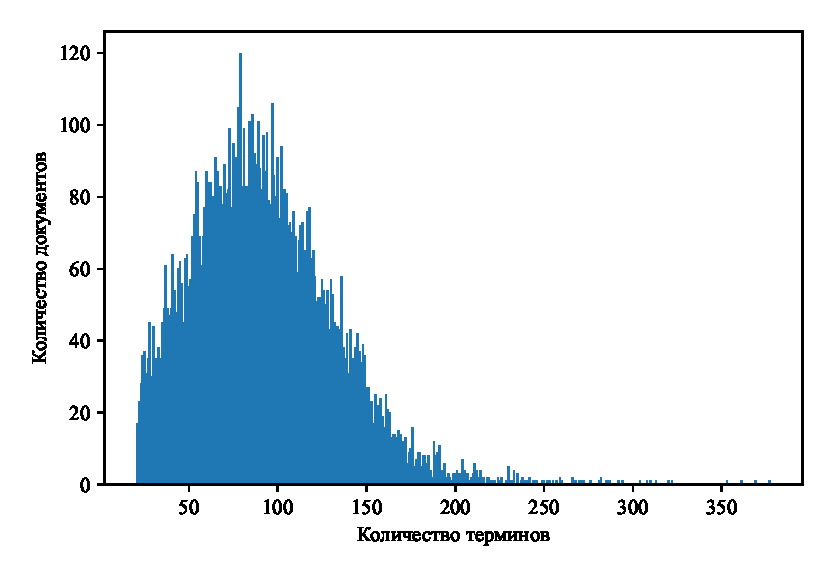
\includegraphics[scale = 0.6]{Pictures/Statistics.eps}}
    \subfloat[Термины, состоящие из одного слова]{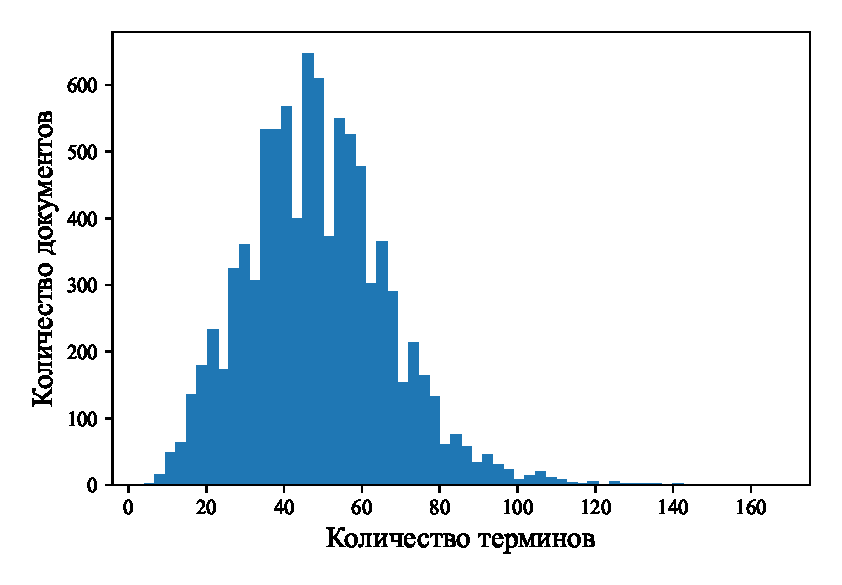
\includegraphics[scale = 0.6]{Pictures/Statistics_1.eps}}
    \caption{Распределение терминов по документам}
    \label{fg:Dataset}
\end{figure}

    Документы представлены в текстовом формате и были получены путём считывания текста из pdf-файлов. Для проведения первого эксперимента из статей удаляются числа, заголовки и ссылки на литературу, затем эксперимент разделяется на два направления: выделение терминов с помощью библиотеки BigARTM и поиск кандидатов в термины с помощью TopMine. Поиск терминов сначала осуществляется в предположении, что они состоят из одного слова.

    Для использования BigARTM необходимо привести слова к нормальной форме. Так как датасет состоит из статей, написанных на английском языке, для этого используется \textit{стемминг} -- отбрасывание окончаний и других изменяемых частей слова. Затем полученные документы собираются в файл формата Vopal Wabbit, который уже обрабатывается с помощью библиотеки BigARTM. Для подбора подходящих гиперпараметров эксперимент запускается с различными комбинациями гиперпараметров сглаживания, разреживания и декоррелирования.

\section{Анализ ошибки}

\section{Заключение}

\bibliographystyle{plain}
\bibliography{references.bib}

\end{document}
